\documentclass[14pt,aspectratio=1610]{beamer}

\usepackage[brazil]{babel}
\usepackage[utf8]{inputenc}
%\UseRawInputEncoding
\usepackage[T1]{fontenc}
%\usepackage{Sweave}
\usepackage{animate}
\usepackage{amsbsy}
\usepackage{amsfonts}
\usepackage{amsmath}
\usepackage{amssymb}
\usepackage{amsthm}
\usepackage[toc,page,title,titletoc]{appendix}
%\usepackage[fixlanguage]{babelbib}
%\usepackage[pdftex]{color}
\usepackage{dsfont}
\usepackage{esvect}
\usepackage[labelfont=bf]{caption}
\usepackage{subcaption}
\usepackage{float}
\usepackage[Glenn]{fncychap}%Sonny %Conny %Lenny %Glenn %Renje %Bjarne %Bjornstrup
%\usepackage{geometry, calc, color, setspace}%
%\geometry{a4paper, headsep=1.0cm, footskip=1cm, lmargin=3cm, rmargin=2cm, tmargin=3cm, bmargin=2cm}
\usepackage{graphicx}
\usepackage{indentfirst}%Para indentar os parágrafos automáticamente
\usepackage{lipsum}
\usepackage{longtable}
\usepackage{mathtools}
\usepackage{listings}%Inserir codigo do R no latex
\usepackage{multirow}
\usepackage{multicol}
\usepackage{csquotes}
\usepackage[maxcitenames=2,terseinits=true,natbib=true, style=authoryear, maxbibnames=99]{biblatex}
\addbibresource{../Referencias/Referencias.bib}
%\usepackage{csquotes}
%\usepackage[natbib=true,style=abnt, sorting=none]{biblatex}
%\addbibresource{bibliografia.bib}
\usepackage[figuresright]{rotating}
\usepackage{spalign}
%\usepackage{pgfpages}
\usepackage{pgfplots}
\pgfplotsset{compat=1.18}
\usepackage{tikz}
\usepackage{color, colortbl}
\usepackage{ragged2e}%para justificar o texto dentro de algum ambiente
\definecolor{Gray}{gray}{0.9}
\definecolor{LightCyan}{rgb}{0.88,1,1}
%\usepackage{grffile}
\usepackage{url}
\usepackage[all]{xy}
\usepackage{hyperref}


%\usetheme{Madrid}
%\usecolortheme[RGB={193,0,0}]{structure}
\usetheme{metropolis}
\definecolor{mycolor}{RGB}{34, 45, 50}
\setbeamercolor{structure}{fg=mycolor}
\usepackage{mathpazo} % Fonte elegante para matemática
\usepackage{helvet} % Fonte sans-serif para texto
\renewcommand{\familydefault}{\sfdefault} % Definir fonte padrão como sans-serif

%\setbeamertemplate{footline}[frame number]
%\setbeamertemplate{footline}[text line]{%
%  \parbox{\linewidth}{\vspace*{-8pt}\hfill\date{}\hfill\insertshortauthor\hfill\insertpagenumber}}
\beamertemplatenavigationsymbolsempty
\renewcommand{\vec}[1]{\mbox{\boldmath$#1$}}
\newtheorem{Teorema}{Teorema}
\newtheorem{Proposicao}{Proposição}
\newtheorem{Definicao}{Definição}
\newtheorem{Corolario}{Corolário}
\newtheorem{Demonstracao}{Demonstração}
\newcommand{\bx}{\ensuremath{\bar{x}}}
\newcommand{\Ho}{\ensuremath{H_{0}}}
\newcommand{\Hi}{\ensuremath{H_{1}}}


\apptocmd{\frame}{}{\justifying}{} % Allow optional arguments after frame.

\title{Estatística I}
\author{Prof. Fernando de Souza Bastos \texorpdfstring{\\ fernando.bastos@ufv.br}{}}
\institute{Departamento de Estatística\texorpdfstring{\\ Universidade Federal de Viçosa}{}\texorpdfstring{\\ Campus UFV - Viçosa}{}}
\date{}
\newcommand\mytext{Aula 4}
\newcommand\mytextt{Fernando de Souza Bastos}
\newcommand\mytexttt{\url{https://ufvest.github.io/}}

\makeatletter
\setbeamertemplate{footline}
{
  \leavevmode%
  \hbox{%
  \begin{beamercolorbox}[wd=.3\paperwidth,ht=2.25ex,dp=1ex,center]{author in head/foot}%
    \usebeamerfont{author in head/foot}\mytext
  \end{beamercolorbox}%
  \begin{beamercolorbox}[wd=.3\paperwidth,ht=2.25ex,dp=1ex,center]{title in head/foot}%
    \usebeamerfont{title in head/foot}\mytextt
  \end{beamercolorbox}%
  \begin{beamercolorbox}[wd=.35\paperwidth,ht=2.25ex,dp=1ex,right]{site in head/foot}%
    \usebeamerfont{site in head/foot}\mytexttt\hspace*{2em}
    \insertframenumber{} / \inserttotalframenumber\hspace*{2ex} 
  \end{beamercolorbox}}%
  \vskip0pt%
}
\makeatother

\providecommand{\arcsin}{} \renewcommand{\arcsin}{\hspace{2pt}\textrm{arcsen}}
\providecommand{\sin}{} \renewcommand{\sin}{\hspace{2pt}\textrm{sen}}
%\newtheorem{Teorema}{Teorema}
%\newtheorem{Proposicao}{Proposição}
%\newtheorem{Definicao}{Definição}
%\newtheorem{Corolario}{Corolário}
%\newtheorem{Demonstracao}{Demonstração}

\titlegraphic{\hspace*{8cm}\href{https://fsbmat-ufv.github.io/}{
\includegraphics[width=2cm]{figs/mylogo.png}}
}


\usepackage{hyperref,bookmark}
\hypersetup{
  colorlinks=true,
  linkcolor=blue,
  citecolor=red,
  filecolor=blue,
  urlcolor=blue,
}

% Layout da pagina
\hypersetup{pdfpagelayout=SinglePage}
\begin{document}
%\input{Aula4-concordance}

\frame{\titlepage}

\begin{frame}{}
\frametitle{\bf Sumário}
\tableofcontents
\end{frame}

\section{Introdução}
\begin{frame}{}
\frametitle{Visualizações Gráficas}
\begin{block}{}
\justifying
Gráficos e tabelas são uma constante em periódicos como jornais diários, revistas, periódicos técnicos e relatórios, acadêmicos ou não. Apesar disso, não existe uma teoria complexa sobre gráficos nos livros de Matemática e/ou Estatística. Na verdade, não existe muita teoria. No entanto, essa é uma parte essencial na formação de qualquer profissional. Na verdade, é essencial para a formação de qualquer cidadão.
\end{block}
\end{frame}

\begin{frame}{}
\frametitle{Visualizações Gráficas}
\begin{block}{}
\justifying
As técnicas, os conceitos e o conteúdo sobre visualizações gráficas fazem parte da Estatística Descritiva e, conforme \cite{unwin}, é parte essencial da Análise de Dados.
\end{block}
\pause
\begin{block}{Estatística Descritiva}
\justifying
A Estatística Descritiva emprega métodos numéricos e gráficos para investigar padrões em um conjunto de dados, resumir informações e apresentar resultados de maneira apropriada. 
\end{block}
\pause
\begin{block}{}
\justifying
Um Gráfico Estatístico é uma representação visual dos dados e, tem a vantagem de, rápida e concisamente, informar sobre sua variabilidade. 
\end{block}
\end{frame}

\begin{frame}{}
\frametitle{Visualizações Gráficas}
\begin{block}{Cuidado!}
\justifying
Existem vários tipos e formatos de gráficos e, tanto a escolha quanto a forma como são visualizados podem ter uma influência importante nas conclusões tiradas em relação a análise dos dados. Não há limites para o número de possibilidades de interpretações. Isso significa que você precisa adquirir ex\-pe\-ri\-ên\-cia na criação e visualização de gráficos para aprender a apreciar o que eles podem e não podem mostrar.
\end{block}
\pause
\begin{block}{}
\justifying
Não é o que você olha que importa, é o que você vê.
\begin{flushright}
Henry David Thoreau
\end{flushright}
\end{block}
\end{frame}

\begin{frame}{}
	\frametitle{Gráficos Enganosos}
	\begin{block}{}
		\justifying
		A utilização de gráficos com escalas truncadas ou manipuladas pode distorcer a percepção dos dados. Por exemplo, iniciar o eixo vertical (y) de um gráfico de barras em um valor diferente de zero pode exagerar diferenças entre categorias que, na rea\-li\-da\-de, são mínimas. 
	\end{block}
\end{frame}


\begin{frame}{Gráficos Enganosos}
	\begin{block}{Cuidado!}
		\centering
		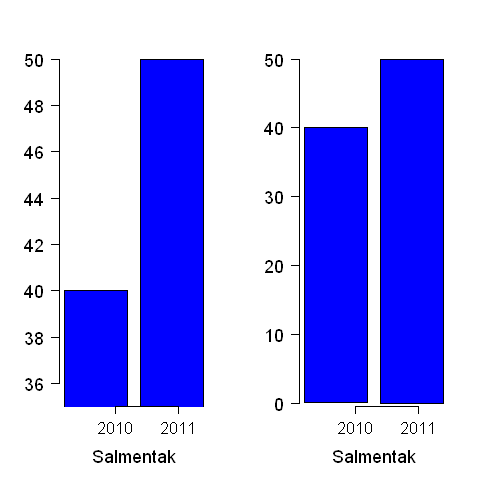
\includegraphics[width=0.5\linewidth]{figs/Enganoso1.png}
		\tiny Fonte: \href{https://pt.wikipedia.org/wiki/Gráfico\_enganoso}{Wikipedia}
	\end{block}
\end{frame}

\begin{frame}{Gráficos Enganosos}
	\begin{block}{Comparativo}
		\centering
		\begin{minipage}{0.48\linewidth}
			\centering
			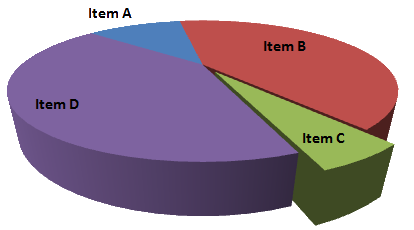
\includegraphics[width=\linewidth]{figs/Enganoso2.png}
			\captionof{figure}{O item C parece ser tão grande quanto o item A e o item D parece muito maior que o item B.}
		\end{minipage}
		\hfill
		\begin{minipage}{0.48\linewidth}
			\centering
			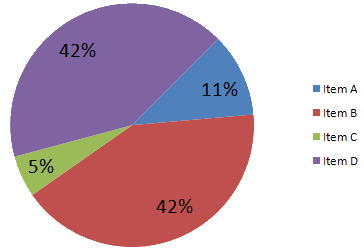
\includegraphics[width=\linewidth]{figs/Enganoso3.png}
			\captionof{figure}{Na realidade, O item C é menos da metade do tamanho do item A. Os itens B e D são do mesmo tamanho.}
		\end{minipage}
	\end{block}
\end{frame}

\begin{frame}{Gráficos Enganosos}
	\begin{block}{Comparativo}
		\centering
		\begin{minipage}{0.48\linewidth}
			\centering
			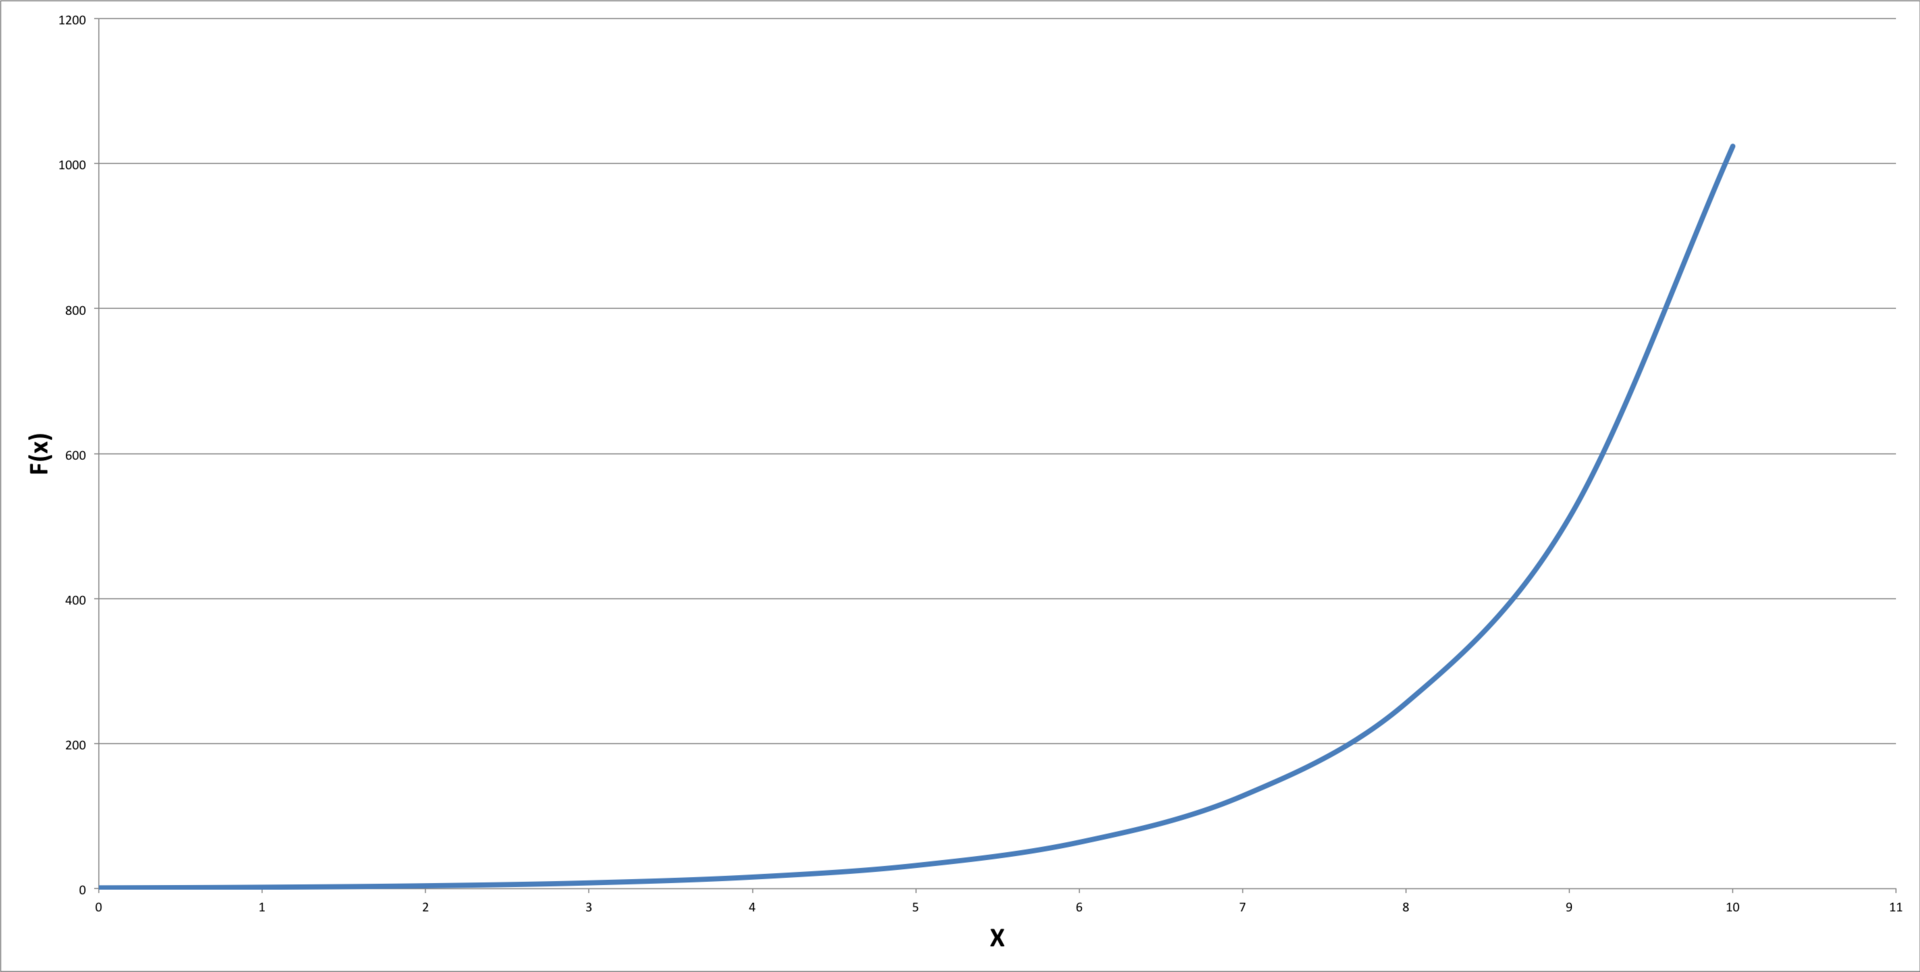
\includegraphics[width=\linewidth]{figs/Enganoso4.png}
			\captionof{figure}{Função exponencial $f(x) = 2^{x}$. Escala linear, mostrando claramente uma tendência exponencial.}
		\end{minipage}
		\hfill
		\begin{minipage}{0.48\linewidth}
			\centering
			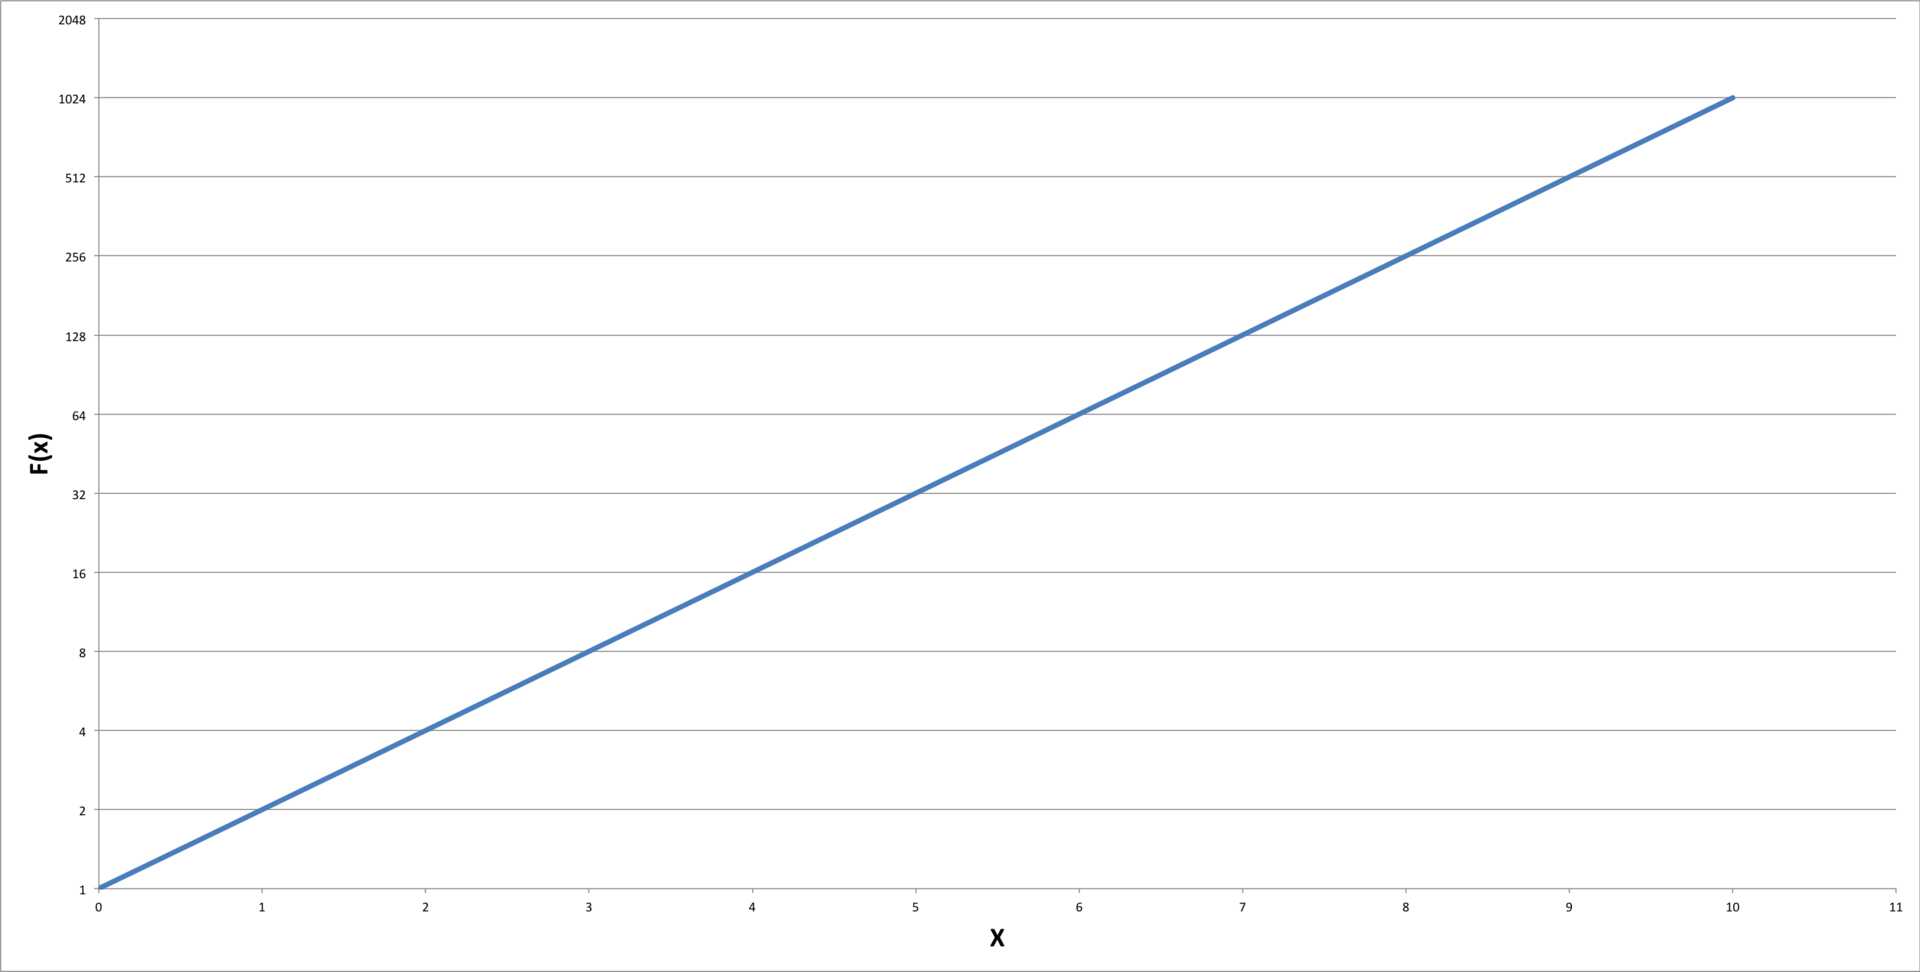
\includegraphics[width=\linewidth]{figs/Enganoso5.png}
			\captionof{figure}{Função exponencial $f(x) = 2^{x}$. Escala logarítmica, mostrando uma linha reta.}
		\end{minipage}
	\end{block}
\end{frame}


\begin{frame}{}
\frametitle{Visualizações Gráficas}
\begin{block}{}
\justifying
A depender do tipo de variável considerada, temos diferentes tipos de gráficos. Veremos alguns a partir de agora!
\end{block}
\end{frame}

\section{Gráficos para Variáveis Qualitativas}
\subsection{Gráfico de Barras}
\begin{frame}{}
\frametitle{Gráfico de Barras}
\begin{block}{}
\justifying
Tomemos como ilustração a variável Y: grau de instrução da Tabela \href{https://raw.githack.com/ufvest/ufvest.github.io/master/Aulas_EST105/CompanhiaMB.html}{CompanhiaMB}. Para organizar os dados provenientes de uma variável qualitativa, é usual fazer uma tabela de frequências, como a Tabela abaixo, antes de construir os gráficos.
\end{block}
\end{frame}

\begin{frame}{}
\frametitle{Distribuições de Frequências}
\vspace{-0.5cm}
\begin{block}{}
\justifying
\begin{table}[H]
\caption{Frequências e porcentagens dos 36 empregados da seção de orçamentos da Companhia MB segundo o grau de instrução.}
\label{tab2}
\begin{tabular}{c|c|c|c}
\hline
Grau de   &Frequência&Proporção&Porcentagem\\
instrução &$n_{i}$   &$f_{i}$  &$100f_{i}$ \\
\hline
Fundamental&12       &0,3333   &33,33      \\
Médio      &18       &0,5000   &50,00      \\
Superior   & 6       &0,1667   &16,67      \\
\hline
Total      &36       &1,0000   &100,00     \\
\hline
\end{tabular}
\subcaption*{\textbf{Fonte:} \cite{morettin2017estatistica}}
\end{table}
\end{block}
\end{frame}

\begin{frame}{}
\frametitle{Gráfico de Barras}
\begin{block}{}
\justifying
O gráfico em barras consiste em construir retângulos ou barras, em que uma das dimensões é proporcional à magnitude a ser representada $(n_{i}\ \textrm{ou}\ f_{i}),$ sendo a outra arbitrária, porém igual para todas as barras. Essas barras são dispostas paralelamente umas às outras, horizontal ou verticalmente. Na próxima Figura temos o gráfico em barras (verticais) para a variável ``Grau de Instrução''.
\end{block}
\end{frame}

\begin{frame}{}
\frametitle{Gráfico de Barras}
\begin{block}{}
\begin{center}
\setkeys{Gin}{width=0.5\linewidth}
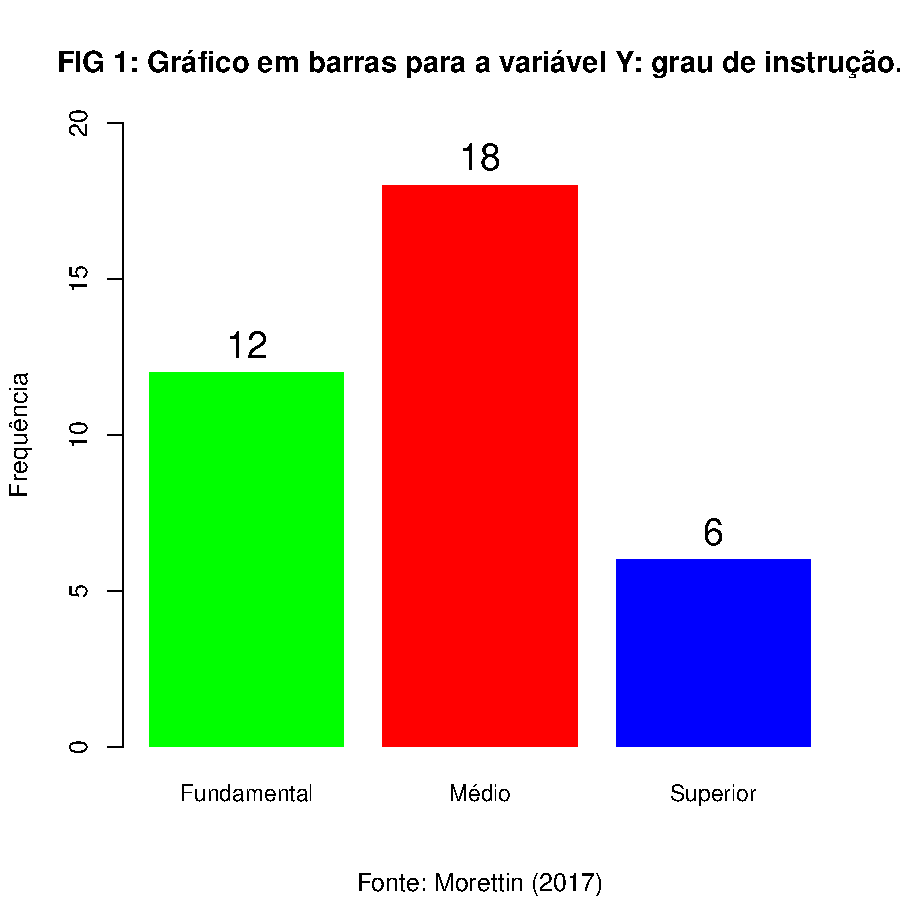
\includegraphics{Aula4-bp1}
\end{center}
% \justifying
% \begin{figure}[H]
%     \centering
%     \includegraphics[scale=0.5]{Fig3}
%     \caption{Gráfico em barras para a variável $Y:$ grau de instrução (\cite{Morettin09}).}
%     \label{Fig3_ex}
%   \end{figure}
\end{block}
\end{frame}

\begin{frame}{}
\frametitle{Gráfico de Barras}
\begin{block}{}
\begin{center}
\setkeys{Gin}{width=0.5\linewidth}
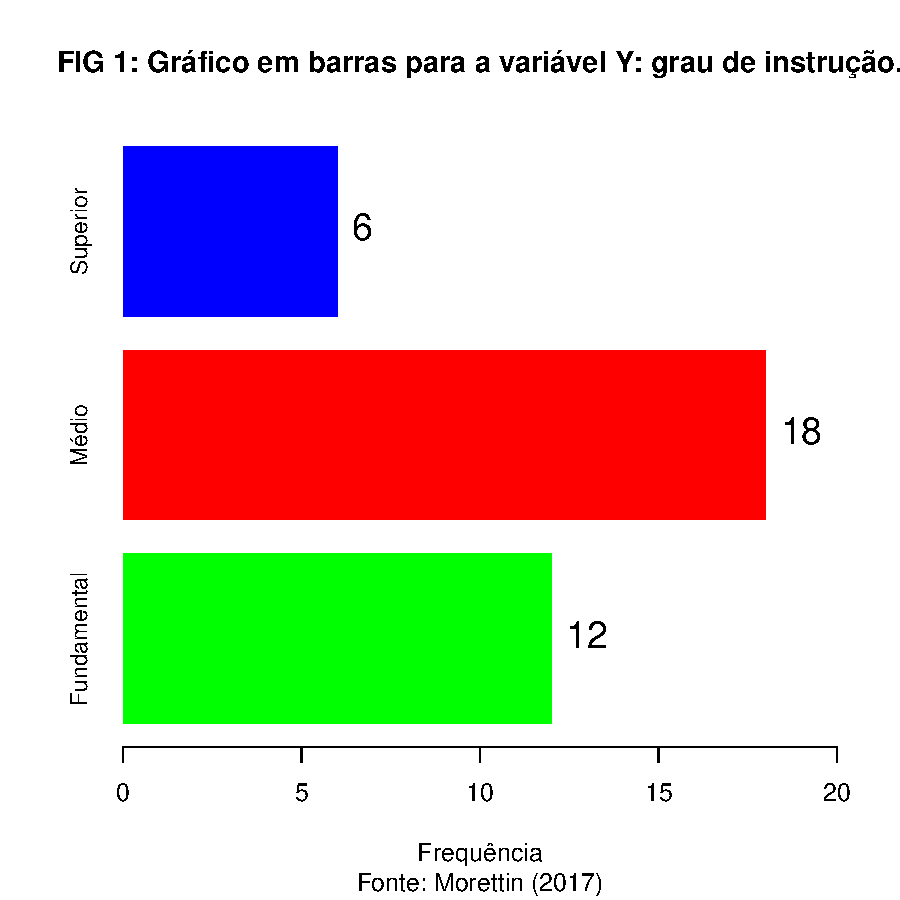
\includegraphics{Aula4-bpHorizontal}
\end{center}
% \justifying
% \begin{figure}[H]
%     \centering
%     \includegraphics[scale=0.5]{Fig3}
%     \caption{Gráfico em barras para a variável $Y:$ grau de instrução (\cite{Morettin09}).}
%     \label{Fig3_ex}
%   \end{figure}
\end{block}
\end{frame}

%\begin{frame}{}
%\frametitle{Gráficos de Barras}
%\begin{block}{}
%\justifying
%O conjunto de dados Fleiss93 do pacote meta contém detalhes de sete estudos sobre o uso de aspirina após infarto do miocárdio. A Figura abaixo representa um gráfico de barras dos tamanhos dos estudos, com os estudos ordenados pelo número total de pacientes. 
%\end{block}
%\begin{block}{}
%\begin{center}
%\setkeys{Gin}{width=0.3\linewidth}
%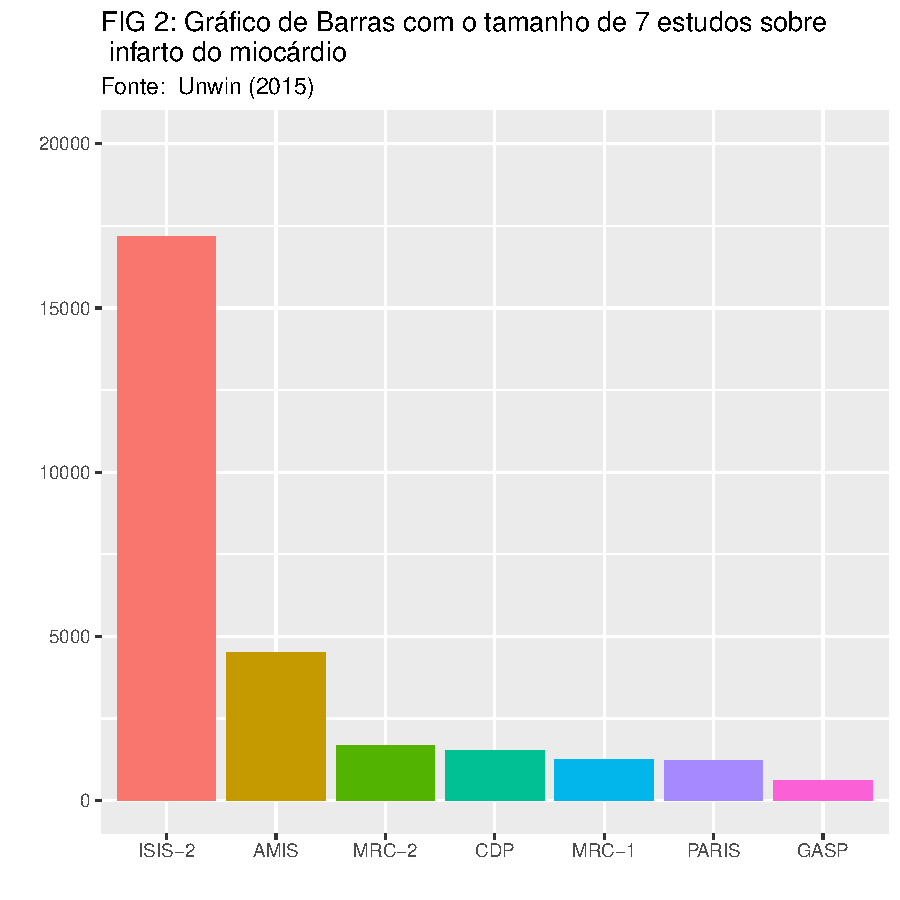
\includegraphics{Aula4-bp2}
%\end{center}
%\end{block}
%\end{frame}

%\begin{frame}{Gráfico de Barras}
%\frametitle{}
%\begin{block}{}
%\begin{center}
%\setkeys{Gin}{width=0.5\linewidth}
%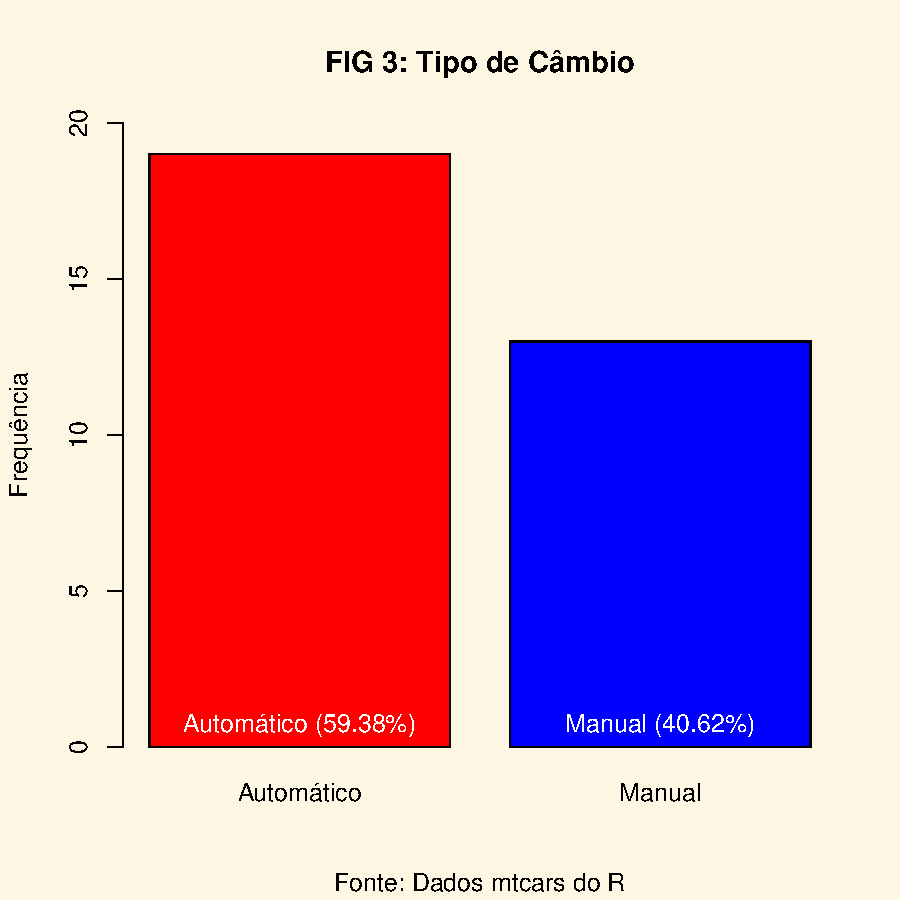
\includegraphics{Aula4-bp3}
%\end{center}
%\end{block}
%\end{frame}

\begin{frame}{}
\frametitle{Gráficos de Barras}
\begin{block}{}
\justifying
Os gráficos de barras são talvez o tipo de visualização de dados mais comumente usado. No entanto, para a representação de variáveis qualitativas, há também o gráfico de setores, popularmente conhecido como gráfico de pizza.
\end{block}
\end{frame}

\subsection{Gráfico de Pareto}
\begin{frame}{}
\frametitle{Gráfico de Pareto}
\begin{block}{}
\justifying
Um gráfico de Pareto é um gráfico de barras em que as barras são ordenadas da maior frequência de ocorrência para a menor frequência de ocorrência. No gráfico de Pareto também acrescentamos uma linha acima das barras com a frequência acumulada da variável.

\end{block}
\end{frame}

\begin{frame}{}
\frametitle{Gráfico de Pareto}
\begin{block}{}
\begin{center}
\setkeys{Gin}{width=0.5\linewidth}
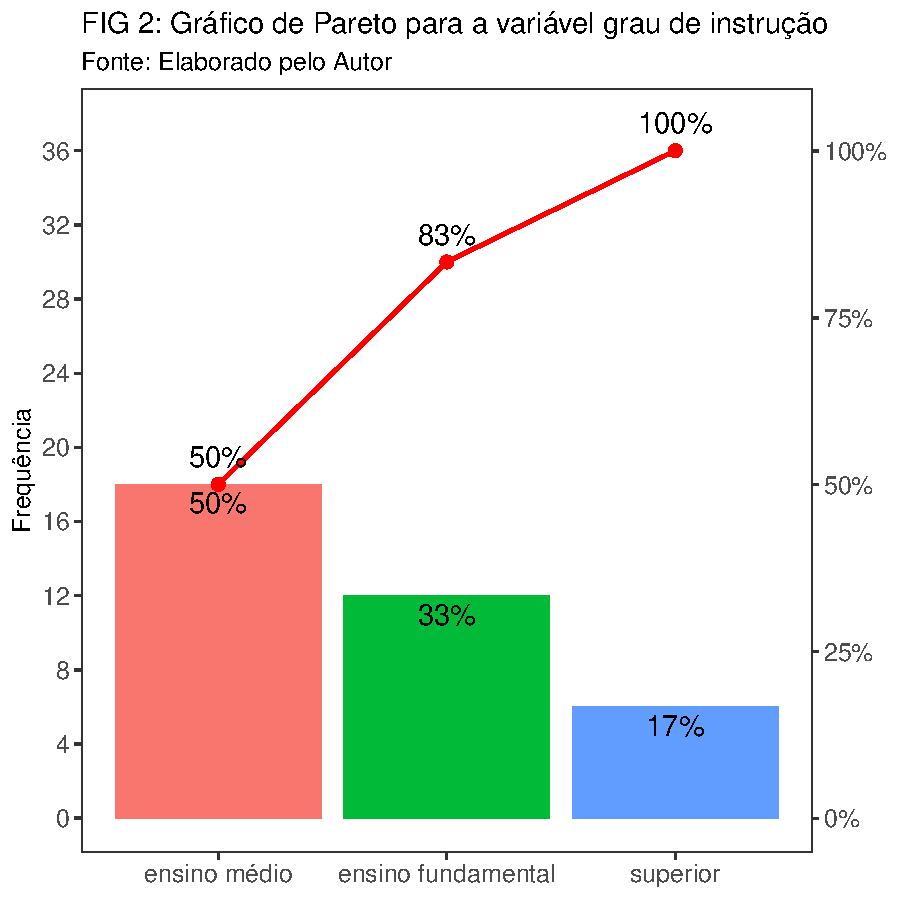
\includegraphics{Aula4-pareto}
\end{center}
% \justifying
% \begin{figure}[H]
%     \centering
%     \includegraphics[scale=0.5]{Fig3}
%     \caption{Gráfico em barras para a variável $Y:$ grau de instrução (\cite{Morettin09}).}
%     \label{Fig3_ex}
%   \end{figure}
\end{block}
\end{frame}

\subsection{Gráfico de Barras Empilhadas}
\begin{frame}{}
\frametitle{Gráfico de Barras Empilhadas}
%\begin{block}{}
\begin{center}
\setkeys{Gin}{width=0.5\textwidth}
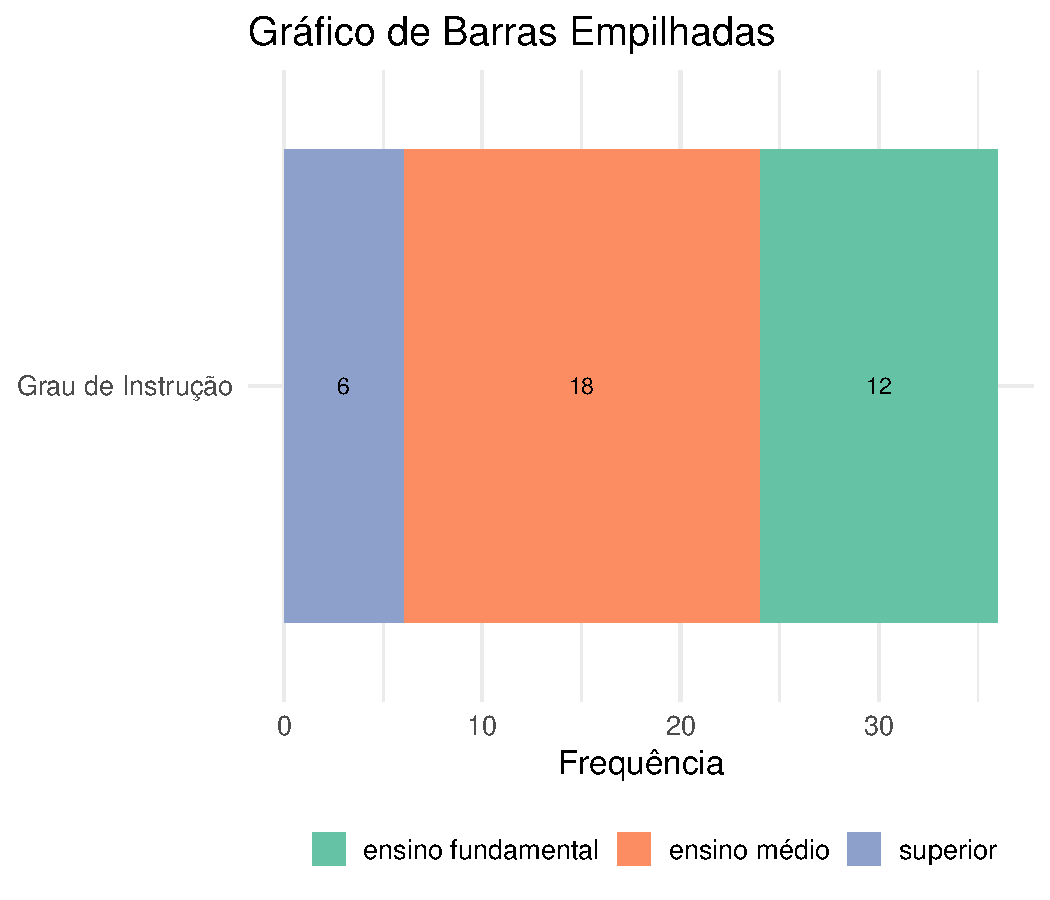
\includegraphics{Aula4-empilhadas}
\end{center}
%\end{block}
\end{frame}

\begin{frame}{}
\frametitle{Gráfico de Barras Empilhadas}
%\begin{block}{}
\begin{center}
\setkeys{Gin}{width=0.5\textwidth}
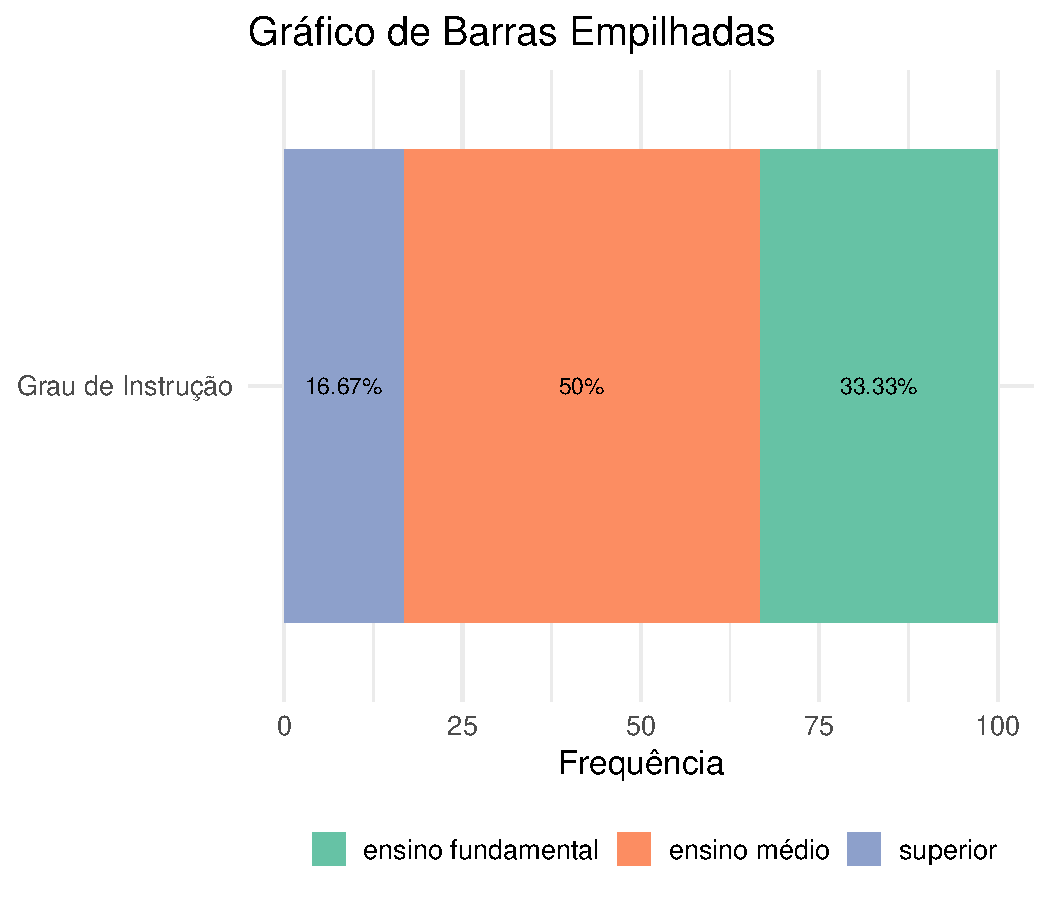
\includegraphics{Aula4-empilhadas2}
\end{center}
%\end{block}
\end{frame}

\subsection{Gráfico de Setores}
\begin{frame}{Gráfico de Setores}
\frametitle{}
\begin{block}{}
\justifying
O gráfico em setores é comumente utilizado para representar parte de um todo, geralmente em percentagens. Ele é bastante apropriado para mostrar frequências de ocorrências de variáveis qualitativas.
\end{block}
\end{frame}

\begin{frame}{Gráfico de Setores}
\frametitle{}
\begin{block}{}
\begin{center}
\setkeys{Gin}{width=0.5\linewidth}
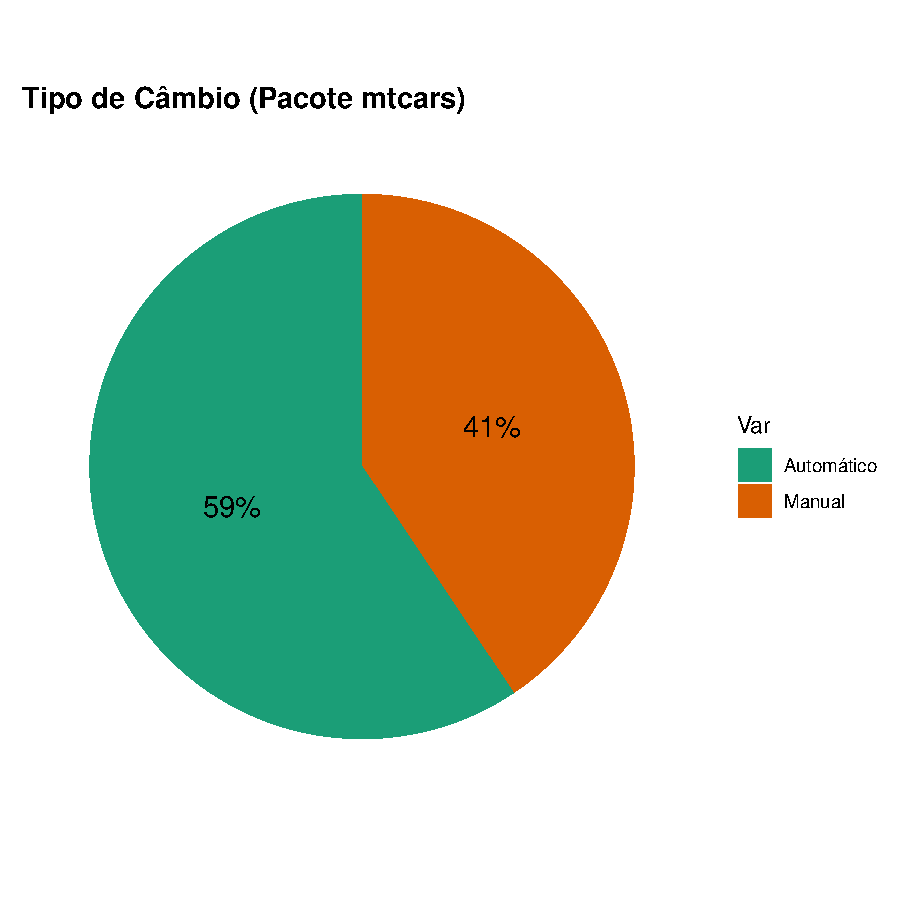
\includegraphics{Aula4-pie1}
\end{center}
\end{block}
\end{frame}

\begin{frame}{}
\frametitle{}
\begin{block}{}
\begin{center}
\setkeys{Gin}{width=0.5\linewidth}
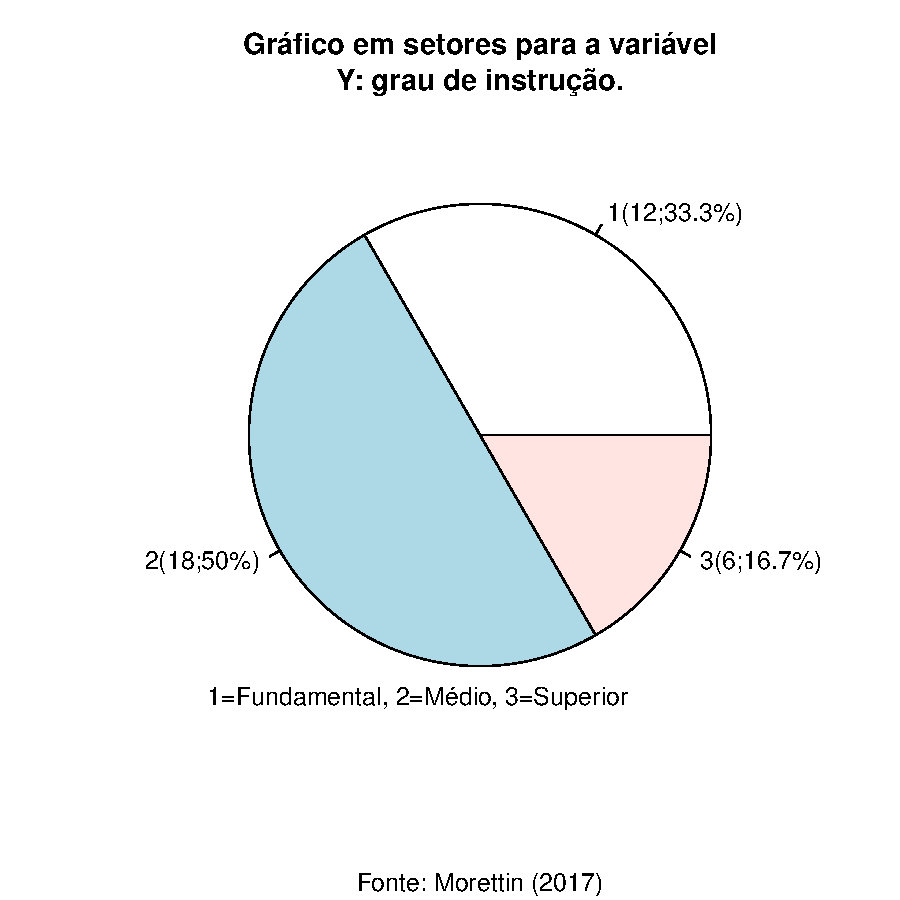
\includegraphics{Aula4-pie2}
\end{center}
\end{block}
\end{frame}

\begin{frame}{}
\frametitle{}
\begin{block}{}
\justifying
Um procedimento alternativo para resumir um conjunto de valores, com o objetivo de se
obter uma idéia da forma de sua distribuição, é o ramo-e-folhas. Uma vantagem deste diagrama é que não perdemos (ou perdemos pouca) informação sobre os dados em si.
\end{block}
\end{frame}

\begin{frame}{}
\frametitle{Diagrama de ramos e folhas para variáveis contínuas}
\begin{block}{}
\justifying
Quando o número de observações é relativamente grande, este diagrama pode ser útil.
\begin{table}[H]
\caption{Diagrama de Ramos e Folhas da idade}
\begin{tabular}{c|ccccccccccccccccc}
Ramo&\multicolumn{17}{c}{Folhas}\\
\hline
2&0&3&5&6&6&7&8&9& & & & & & & & & \\
3&0&1&1&2&2&3&3&4&4&5&5&6&6&7&7&8&9\\
4&0&0&1&1&2&3&3&4&6&8& & & & & & & 
\end{tabular}
\end{table}
\end{block}
\end{frame}

\begin{frame}{}
\frametitle{}
\small
\begin{block}{}
\justifying
\begin{table}[H]
\caption{Diagrama de Ramos e Folhas dos Salários ($\times$ sal. Min)}
\scalebox{0.6}{%
\begin{tabular}{c|cccccccc}
Ramos&\multicolumn{8}{c}{Folhas}\\
\hline
 4&& 00&& 56&&   &&   \\
 5&& 25&& 73&&   &&   \\
 6&& 26&& 66&& 86&&   \\
 7&& 39&& 44&& 59&&   \\
 8&& 12&& 46&& 74&& 95\\
 9&& 13&& 35&& 77&& 80\\
10&& 53&& 76&&   &&   \\
11&& 06&& 59&&   &&   \\
12&& 00&& 79&&   &&   \\
13&& 23&& 60&& 85&&   \\
14&& 69&& 71&&   &&   \\
15&& 99&&   &&   &&   \\
16&& 22&&   && 61&&   \\
17&& 26&&   &&   &&   \\
18&& 75&&   &&   &&   \\
19&& 40&&   &&   &&   \\
20&&   &&   &&   &&   \\
21&&   &&   &&   &&   \\
22&&   &&   &&   &&   \\
23&&   && 30&&   &&   \\
\end{tabular}}
\end{table}
\end{block}
\end{frame}

\begin{frame}{}
\frametitle{}
\begin{block}{}
\justifying
Algumas informações que se obtêm deste ramo-e-folhas são:
\begin{enumerate}
\item \justifying Há um destaque grande para o valor 23,30.\pause
\item \justifying Os demais valores estão razoavelmente concentrados entre 4,00 e 19,40.\pause
\item \justifying Um valor mais ou menos típico para este conjunto de dados poderia ser, por 
exemplo, 10,00.\pause
\item \justifying Há uma leve assimetria em direção aos valores grandes; a suposição de que estes dados possam ser considerados como amostra de uma população com distribuição simétrica, em forma de sino (a chamada distribuição normal), pode ser questionada.
\end{enumerate}
\nocite{Morettin09, Apostila, eric, montgomery2016, Bastos2025}
\end{block}
\end{frame}

\begin{frame}[allowframebreaks]
\frametitle{}
\printbibliography
\end{frame}


\end{document}
